\documentclass[oneside,a4paper,12pt]{article}
\usepackage{graphicx}
\usepackage[section]{placeins}
\usepackage{listings}
\graphicspath{{~/templates/}, {../images/}}

\usepackage{hyperref}
\hypersetup{
	colorlinks=true,
	linkcolor=black,
	filecolor=magenta,      
	urlcolor=blue,
	pdftitle={Overleaf Example},
	pdfpagemode=FullScreen,
}

\usepackage{breakurl}


\makeindex
\begin{document}
	\begin{titlepage}
		\includegraphics[width=4cm]{logopopo.png}
		\hspace*{\fill}
		\includegraphics[width=6cm]{univlille.png}
		
		\begin{center}
			\vspace{1cm}
			\textbf{Projet S7}\\
			\textbf{Conception et commande d'un mini Segway}\\
			\vspace{1cm}
			\textbf{Etudiants}\\
			\textbf{Ayman MOUMMADI, Logan PAQUIN}\\
			\textbf{Maxence NEUS, Omar SIFA}\\
			\vspace{2cm}
			
			\textbf{Tuteurs}\\
			\textbf{Mr Midzodzi Pekpe, Mr Othman Lakhal}\\
			
			%\includegraphics[width=13cm]{titlepage.png}\\
			\vspace{\fill}
			\textbf{Janvier 2022}\\
		\end{center}
	\end{titlepage}
	
	\newpage
	\vspace{\fill}
	\paragraph{Résumé}\paragraph{}
	
	Notre sujet se nomme “Conception et commande d’un segway”. Nous devons réaliser un segway miniature et le contrôler à distance. Autrement dit, identifier les composants nécessaires pour la fabrication du segway et le concevoir au Fabricarium de Polytech Lille.
	
	Ce rapport présente l’avancement final de notre projet. Il reprend les parties abordées au semestre 6, en apportant ce qui à été ajouté lors du semestre 7. Il présente également ce que nous n’avons pas pu réaliser, ainsi que comment nous aurions pu effectuer ces tâches.
	
	\vspace{\fill}
	\paragraph{Abstract}\paragraph{}
	
	Our subject is called "Design and control of a segway". We have to make a miniature segway and remote it. In other words, identify the necessary components for the manufacture of the segway and conceive it at the Fabricarium of Polytech Lille.
	
	This wiki report presents the final progress of our project. It takes the parts tackled in the past semester (S6), and adds all that have been done since. Then it describes what we could not do, how we would have done those tasks and why we didn’t.
	\vspace{\fill}
	
	\newpage
	\tableofcontents
	
	
	\newpage
	
	\section{Introduction}
	
	\paragraph{Présentation du projet}\paragraph{}
	
	Notre projet consiste à réaliser un Segway miniature et à le contrôler à distance. Un Segway est un gyropode, soit un véhicule électrique monoplace, constitué d’une plateforme munie de deux roues parallèles sur laquelle l’utilisateur se tient debout, d’un système de stabilisation gyroscopique.

	Nous allons créer les schémas électriques et identifier les composants nécessaires à la fabrication du Segway puis le concevoir au Fabricarium de Polytech. Ensuite nous allons programmer différentes commandes pour gérer le Segway. Cela inclut un contrôle à distance ,puis l’implémentation d’un programme de pilotage autonome à l’aide d’une caméra incluse sur le système.

	\newpage
	
	\section{Cahier des charges}
	
	Le système que nous devons réaliser étant une version miniature d’un Segway, les attentes sont différentes. Alors que le Segway à pour vocation d’offrir un moyen de transport personnel et agile en milieu urbain, notre système doit pouvoir être piloté par l’utilisateur à distance.\\
	
	De plus, notre système est prévu pour une utilisation en intérieur rendue possible grâce à sa taille modeste, mais peut-être amené à évoluer pour une utilisation en extérieur moyennant notamment l’ajout d’une carcasse permettant une isolation contre les liquides et la poussière suffisante.
	
	\begin{figure}[h]
		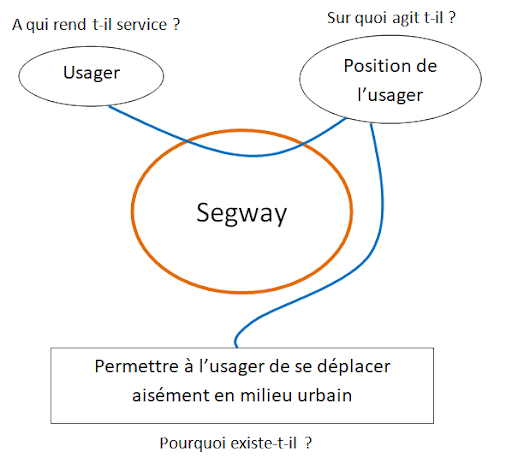
\includegraphics[width=7cm]{bete_corne_segway.png}
		\hspace{0cm}
		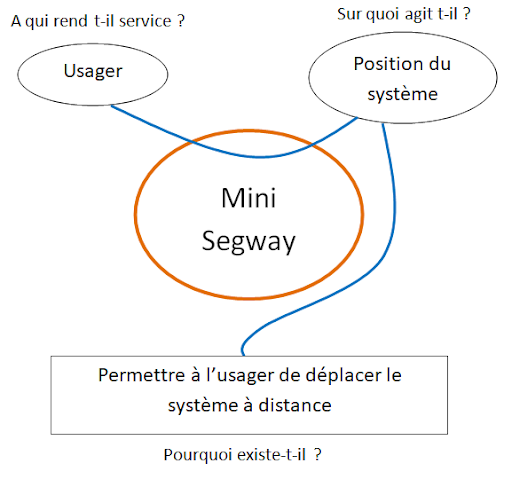
\includegraphics[width=7cm]{bete_corne_mini.png}
		\hspace*{1cm}
		\textbf{Bête à corne du Segway}
		\hspace*{1cm}
		\textbf{Bête à corne de notre Système}
		
		\caption{Bêtes à corne}
	\end{figure}

	Notre système évolue donc dans un environnement simple, ce qui permet de limiter la complexité des contraintes.
	Voici le diagramme pieuvre décrivant les contraintes auxquelles devra répondre notre système.
	

	
	\begin{figure}[h]
		\centering
		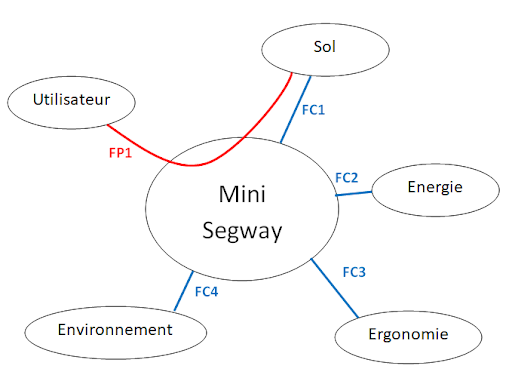
\includegraphics[width=10cm]{pieuvre.png}
		
		\begin{tabular}{|p{1cm}|p{10cm}|}
			\hline
			FP1 & Se déplacer par rapport au sol conformément aux commandes envoyées par l’utilisateur à distance.\\
			\hline
			FC1 & Se tenir en équilibre vertical par rapport au sol en toute circonstance.\\
			\hline
			FC2 & Avoir une autonomie en énergie suffisante.\\
			\hline
			FC3 & Être de taille modeste et facilement transportable.\\
			\hline
			FC4 & Se déplacer en intérieur\\
			\hline
		\end{tabular}		
		
		\caption{Description des besoins}
	\end{figure}

	\begin{figure}[h]
		\centering
		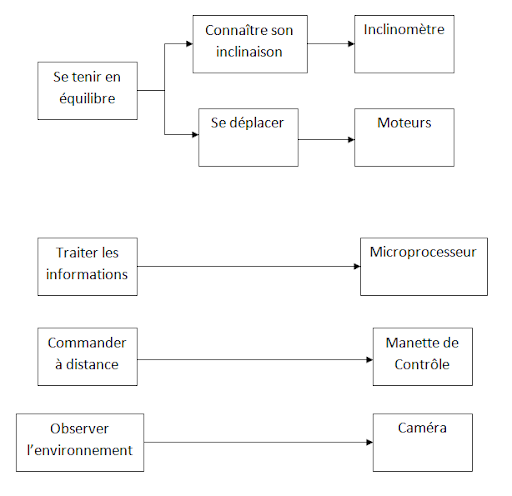
\includegraphics[width=14cm]{shema_fonctionnel.png}
		\caption{Schéma fonctionnel de notre système}
	\end{figure}

	\section{Etat de l'art}
	\paragraph{}
	Le début du 21ème siècle aura été chargé en innovations technologiques en tout genre. Parmi elles, le Segway semble clairement avoir fait l’une des entrées les plus fracassantes sur le marché. En 2001, le premier Segway de Dean Kamen promettait alors de révolutionner la mobilité urbaine avec une sortie de scooter à deux roues auto équilibré, capable d’être piloté par la seule force de sa pensée, ou presque. Vous connaissez le principe : le Segway peut être piloté via une simple inclinaison du corps dans un sens comme dans l’autre.
	\paragraph{}
	Hélas, malgré la révolution annoncée – jusqu’à s’attirer les éloges d’un certain Steve Jobs à sa présentation – le Segway n’a pas réussi à trouver sa place parmi le trafic urbain, alors que les villes l’ont peu à peu banni de leurs routes. La Segway original a alors été relégué au rang de gadget onéreux, mais n’a pas trouvé sa place chez le grand public. Malgré l’échec du premier modèle, la technologie d’auto-équilibrage apportée par le Segway original a subsisté dans bien d’autres produits : Dean Kamen, créateur de l’engin, a finalement vendu son Segway à l’entreprise chinoise Ninebot en 2015. Celle-ci n’a pas manqué de décliner le concept en une multitude de produits, et notamment, des engins moins onéreux et plutôt destinés aux jeunes, tels que ceux qu’on appelle aujourd’hui hoverboard.\\
	
	\sloppy
	\url{https://www.journaldugeek.com/2020/06/24/premier-segway-tire-reverence-pourquoi-manquer/}
	
	\newpage
	
	\section{Organisation}
	
	\subsection{Planning}
	
	Pour pouvoir nous organiser au mieux, nous avons fait un GANTT (comme au S6) qui met des “deadlines” pour chaque partie du projet. Ci-dessous le GANTT prévisionnel qu’on a réalisé au début de semestre.
	
	\begin{figure}[h]
		\centering
		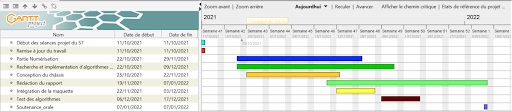
\includegraphics[width=14cm]{gant1.png}
		\caption{GANTT prévisionnel}
	\end{figure}

	Afin d’être critique et pouvoir expliquer les tâches faites à temps et celles où ce n'est pas le cas, nous avons fait un GANTT réel (voir ci-dessous).
	
	\begin{figure}[h]
		\centering
		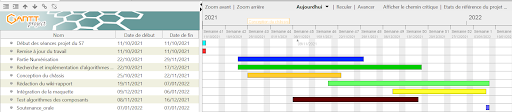
\includegraphics[width=14cm]{gant2.png}
		\caption{GANTT réel}
	\end{figure}

	On peut remarquer qu’on a plus ou moins respecté le GANTT fixé au début avec quelques retards dûs principalement au non fonctionnement de notre accéléromètre qu’on a dû changer et aussi les moteurs pas à pas qui ne fonctionnent pas bien.
	
	\newpage
	
	\subsection{Répartition des tâches}
	
	On s’est réparti les tâches au début de semestre comme suivant:
	
	\begin{itemize}
		\item[Maxence] Programmation
		\item[Omar et Ayman] Recherche bibliographique
		\item[Logan et Omar] Modélisation du segway
		\item[Ayman] Rédaction des suivis sur le WIKI
	\end{itemize}
	
	Néanmoins, à la fin de chaque séance du projet, chacun montrait son avancée et ce qu’il a pu faire durant la séance.
	
	\newpage

	\section{Conception de la commande}
	\label{Conception de la commande}
	
	\subsection{Modélisation du Segway}
	
	La régulation d’inclinaison du Segway consiste à maintenir la consigne $ \psi_{c}(t) $ nulle. Cette régulation est réalisée si, quelle que soit l’inclinaison $ \alpha(t) $ du conducteur, la sortie $ \psi(t) $ converge vers $ \psi_{c}(t) $ , valeur nulle ici. Le conducteur agit directement sur la valeur $ \alpha(t) $ de pour accélérer ou décélérer. Pour le système Segway, conducteur exclu, le paramètre peut être considéré comme une perturbation. Le schéma-bloc fonctionnel du Segway est donc le suivant:
	
	\begin{figure}[h]
		\centering
		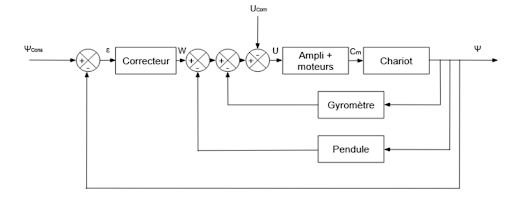
\includegraphics[width=13cm]{shema_bloc_1.png}
		\caption{Schéma bloc du Segway}
	\end{figure}
	
	Il est composé de différents éléments :\\
	Un correcteur, pour réguler la commande\\
	L’ensemble ampli + moteurs qui délivre un couple $ C_{m}(p) = K.U(p) $\\
	L’ensemble chariot + conducteur (le système mécanique) modélisé par l’équation $ \chi(p) = \psi(p) - \alpha(p) = F(p)U(p) - \alpha(p) $\\
	avec :
	
	$$ F(p) = \frac{\frac{2(B+DR)}{RDC}}{\frac{(DA+B^{2})}{DC}p^{2}-1} $$

	A=90kg.m²
	B=75kg.m
	C=750kg.m²/s²
	D=125kg 
	R=240mm\\
	
	(ces valeurs seront expliquées dans la partie juste après)\\
	Le gyromètre : $ u_{g}(t) = k_{g}\frac{d\psi(t)}{dt} $ soit $ U_{g}(p) = pk_{g}\psi(p) $ \\
	Le pendule : $ u_{p}(t) = k_{p}\psi(t) $ soit $ U_{p}(p)=k_{p}\psi(p) $
	
	Nous avons choisi de prendre comme valeurs initiales pour le segway (l’ensemble conducteur + chariot) les valeurs fournies dans ces tableaux, accompagnées des matrices d’inerties correspondantes au système étudié:
	

	\begingroup
	\centering
	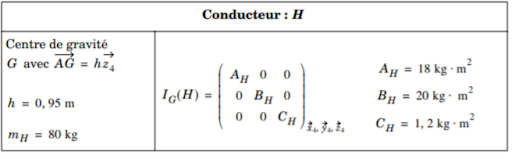
\includegraphics[width=\columnwidth]{tab1.png}
	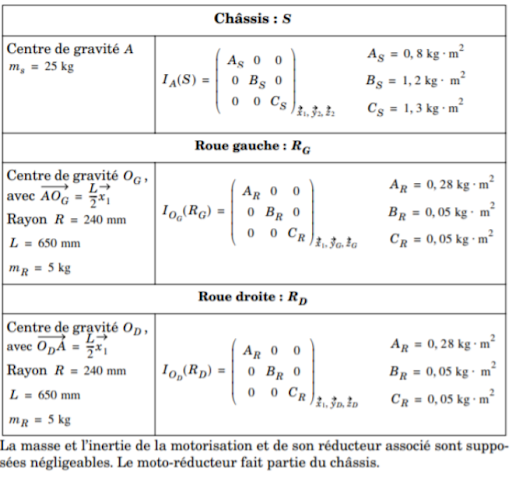
\includegraphics[width=\columnwidth]{tab2.png}
	\endgroup
	
	C’est ainsi que l’on trouve les valeurs de A, B, C, D et R (rayon d’une roue) pour l’ensemble du système mécanique modélisé par l’équation $ \chi(p) = \psi(p) - \alpha(p) = F(p)U(p) - \alpha(p) $
	
	avec :
	
	$$ F(p) = \frac{\frac{2(B+DR)}{RDC}}{\frac{(DA+B^{2})}{DC}p^{2}-1} $$
	
	On a en effet les équations suivantes:
	
	
	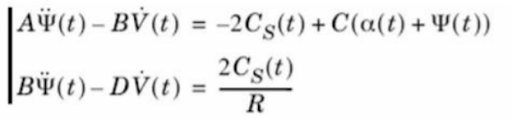
\includegraphics[width=8cm]{cp1.png}
	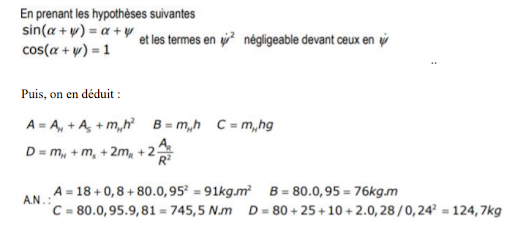
\includegraphics[width=\columnwidth]{cp2.png}
	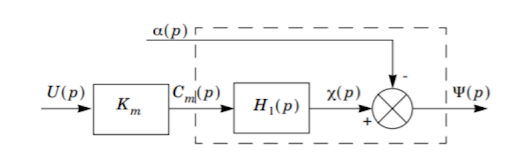
\includegraphics[width=\columnwidth]{cp3.png}
	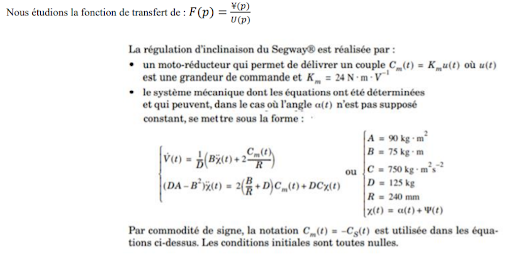
\includegraphics[width=\columnwidth]{cp4.png}
	
	Les conditions sont toutes nulles, nous obtenons à partir la seconde équation différentielle dans Laplace(ci-dessus), l’équation suivante : 
	
	$$ ((DA-B^{2})p^{2}-DC)\chi(p) = 2(\frac{B}{R}+D)C_{m}(p) $$
	
	Nous avons $ H_{1}(p) = \frac{\chi(p)}{C_{m}(p)}$ d’après le schéma bloc ci-dessous.\\
	Nous en déduisons :
	
	$$ H_{1}(p)=\frac{2(\frac{B}{R}+D)C}{(DA+B^{2})p^{2}-DC} = \frac{\frac{2(\frac{B}{R}+D)C}{DC}}{\frac{DA-B^{2}}{DC}p^{2}-1} = \frac{2(\frac{B+DR}{RDC})}{\frac{DA-B^{2}}{DC}p^{2}-1}$$
	Le schéma bloc se justifie alors en écrivant :
	$$ \psi(p) = \chi(p) = K_{m}H_{1}(p)U(p) $$
	
	Le système d’entrée $ u(t)$ et de sortie $\psi(t)$ est instable car le dénominateur de la fonction de transfert possède un pôle réel positif.
	
	$$ p=\pm\sqrt{\frac{DC}{DA-B^{2}}} $$
	avec 
	
	$$ \frac{DA-B^{2}}{DC}=0.06 > 0$$
	
	Nous déterminons les conditions sur $K_{v}$ et $K_{p}$ pour que le système soit stable cette fois-ci avec $\alpha = 0$ (Voir schéma ci-dessous)
	
	$$ \frac{\psi(p)}{W(p)} = \frac{\frac{K_{m}H_{1}(p)}{1+pK_{v}K_{m}H_{1}(p)}}{1+K_{p}\frac{K_{m}H_{1}(p)}{1+pK_{v}K_{m}H_{1}(p)}} = \frac{K_{m}H_{1}(p)}{1+pK_{v}K_{m}H_{1}(p)+K_{p}K_{m}H_{1}(p)} = \frac{K_{s}}{\frac{p^{2}}{\omega^{2}}+pK_{v}K_{s} + K_{p}K_{s}-1}$$
	
	C’est un système de degré 2 qui est stable si et seulement si les coefficients des puissances de p sont différents de 0 et sont de même signe.\\
	Ceci implique : $K_{p} > \frac{1}{K_{s}} $ et $ K_{v}>0 $ pour que le système soit stable.
	
	\subsection{Conversion Numérique}
	
	Dans cette partie nous avons ajouté un CAN dont le but de modéliser notre segway miniature
	
	\begin{figure}[h]
		\centering
		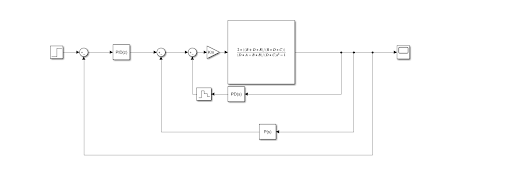
\includegraphics[width=\columnwidth]{shema_bloc_2.png}
		\caption{Schéma bloc du mini Segway}
	\end{figure}
	
	Nous allons maintenant vérifier le comportement de notre Segway miniature afin de nous assurer de son bon fonctionnement. Nous allons pour cela analyser sa réponse pour une consigne d’angle de 1.57 rad (soit un angle de 90°), puis essayer de la corriger avec un régulateur
	
	\begin{figure}[h]
		\begingroup
		\centering
		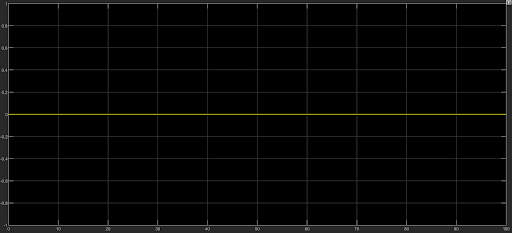
\includegraphics[width=\columnwidth]{matlab1.png}
		\caption{Sans correcteur}
		\endgroup
		\vspace{0.5cm}
		Nous pouvons voir que l’erreur est très grand, en effet le système ne démarre pas.
	\end{figure}
	\begin{figure}[h]
		\begingroup
		\centering
		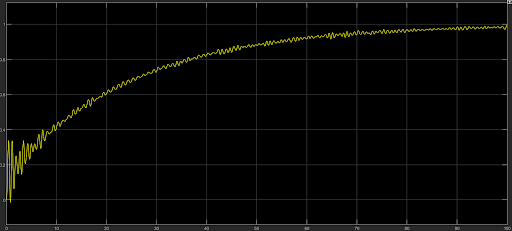
\includegraphics[width=\columnwidth]{matlab2.png}
		\caption{P=1.9 et I=0.9}
		\endgroup
		\vspace{0.5cm}
		Nous remarquons que le système a une erreur plus petite mais le temps de réponse est grand, des oscillations dans les 5 premières secondes.
	\end{figure}
	\begin{figure}[t]
		\begingroup
		\centering
		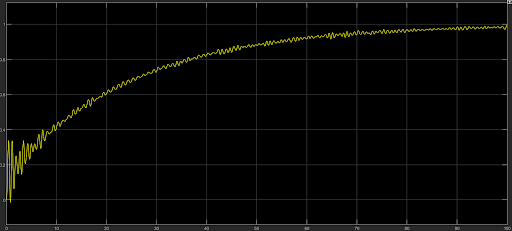
\includegraphics[width=\columnwidth]{matlab2.png}
		\caption{P=1.2 et I=0.5 (Optimisé par Matlab)}
		\endgroup
		\vspace{0.5cm}
		Nous remarquons que le temps de réponse est réglé ainsi la diminution des oscillations.
	\end{figure}

	\section{Conception de la maquette}
	
	\subsection{Concept de base}
	
	Dans sa forme la plus simple, un segway est composé de trois éléments:
	
	\begin{itemize}
		\item un moyen de déterminer l'angle entre le segway et la verticale.
		\item une motorisation permettant un déplacement horizontal.
		\item un algorithme de commande qui réalise un asservissement en position. 
	\end{itemize}

	Pour notre application, on se focalise d'abord sur la stabilisation autonome du segway et le déplacement de celui-ci est prévu dans un second temps. Le but est de déveloper un MVP (Minimum Viable Product) avant d'augmenter la complexité du projet par la suite pour le pousser un peu plus loin.
	
	\subsection{Architecture matérielle}
	\label{Architecture matérielle}
	
	Notre planification pour la conception du segway a quelque peu changée depuis le rapport du S6, en effet nous nous sommes rendus compte que l'utilisation d'une raspberry pi pour gérer l'asservissement ne serai pas possible à cause de l'architecture du processeur qui n'est pas temps réel. Cela rends toute tentative de commande par ce biais irréalisable.\\
	Nous avons donc fait le choix d'abandonner le code existant pour passer sur une architecture d'Arduino utilisant FreeRTOS comme on a pu l'utiliser dans le cadre du module de Systèmes Temps Réels. Nous détaillerons les implications de ce changement dans la partie  \ref{subsection:Architecture logicielle}.
	
	En ce qui concerne la mécanique du segway, nous utilisons toujours deux moteurs pas à pas pour entraîner les deux roues du segway. Ceux-ci sont fixés dans un châsis réalisé par impression 3D.
	
	\newpage
	
	\begin{figure}[h]
		\centering
		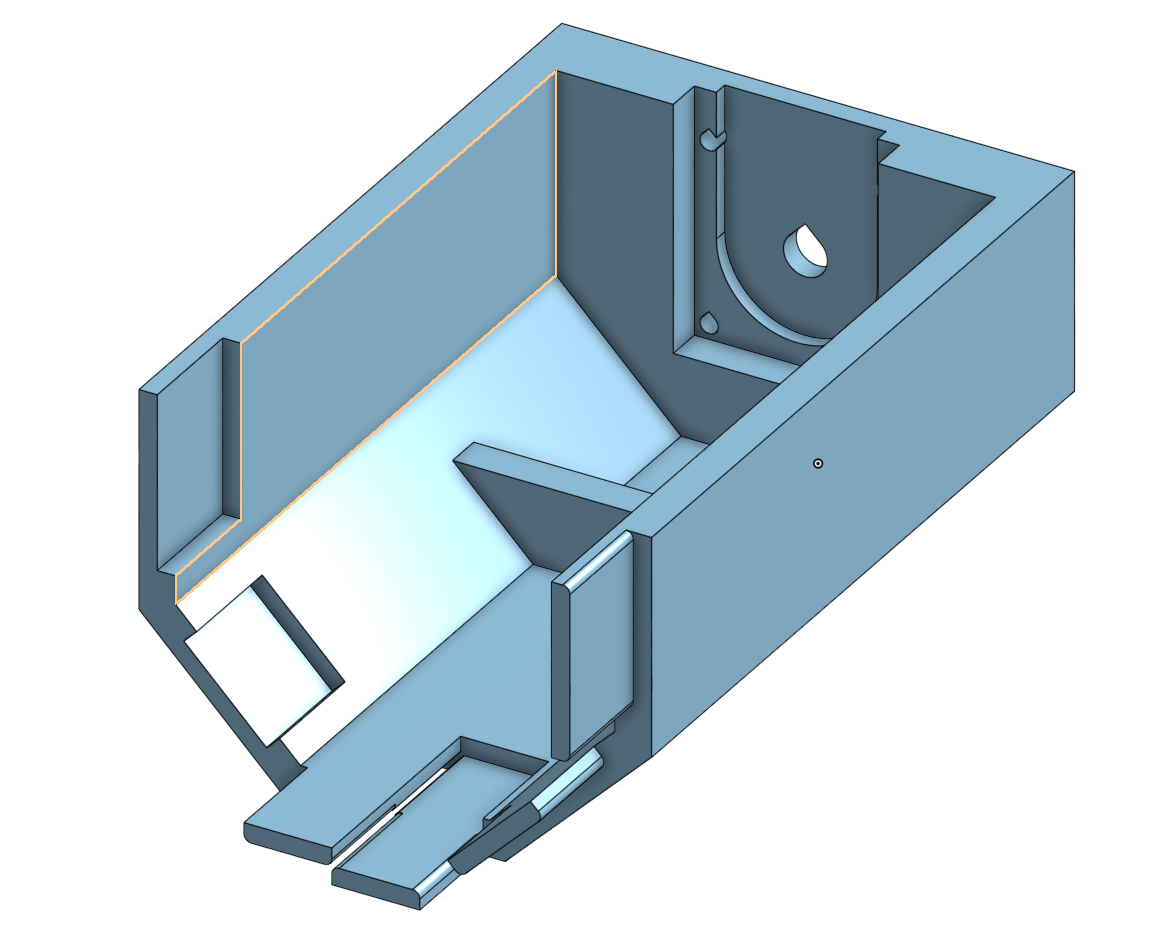
\includegraphics[width=12cm]{CAD_chasis.png}
		\caption{Modèle d'un  demi châsis}
	\end{figure}

	L'électronique ayant beaucoup changé au cours du projet, il n'est pas prévu de fixations pour les composants dans le châsis, mais il reste possible de les y déposer pour fermer le segway.
	
	\subsection{Architecture logicielle}
	\label{subsection:Architecture logicielle}
	
	Comme discuté en \ref{Architecture matérielle} nous avons complétement repris la conception logicielle à zéro avec FreeRTOS, le but étant de créer des processus pour :
	
	\begin{itemize}
		\item[1] Lire la mesure d'angle de l'inclinomètre via une connexion I2C.
		\item[2] Calculer la commande à appliquer aux moteurs grâce aux algorithmes discutés en \ref{Conception de la commande}
		\item[3] Réaliser la commande des moteurs
	\end{itemize}
	
	Le processus 1 peut être facilement dérivé des exemples de lecture d'angle du MPU 6050 disponible avec la bibliothèque Arduino associée.\\
	En revanche un problème apparait pour la commande des moteurs, en effet bien que la commande des moteurs pas à pas permette de facilement faire tourner le moteur d'un certain nombre de pas, cette commande devient difficile lorsque l'on veut réaliser des mouvements de quelques pas à intervale réguliers.
	
	Avec ce type de commande, il semble que le moteur ne soit pas alimenté suffisament longtemps pour réaliser la séquence de commande permettant d'effectuer un pas. En effet les temps d'activation requis pour avoir une commande propre du moteur sont trés précis et il semble que l'Arduino n'arrive pas à suivre avec un temps d'échentillonage assez faible pour avoir une commande efficace. Et ce même avant de l'intégrer dans l'architecture FreeRTOS avec les autres processus qui prendront du temps processeur que l'on a déjà pas.
	
	Le processus 2 de calcule de commande se base sur la représentation en transformée en Z de la chaîne d'asservissement dévellopée en \ref{Conception de la commande}. La conception de celui-ci a été retardée par les problèmes survenus dans la commande des moteurs et reste donc à réaliser.
	
	\subsection{Changements à apporter}
	
	Il semble nécessaire pour régler les problèmes décrits en \ref{subsection:Architecture logicielle} de revoir à nouveau l'architecture pour utiliser des contrôleurs plus avancés pour les moteurs afin de réussir à les commander assez rapidement pour avoir un asservissement correct. Cela pourra passer par l'utilisation de contrôleurs différents ou bien par la séparation physique des parties de commande et de calculs par l'utilisation par exemple d'un microcontrôleur dédié à la commande de chaque moteur que l'on pourra coder en assembleur pour réduire le temps d'execution du C. Plus de recherches à ce sujet seront nécessaires au S8.
	
	
	\newpage
	
	\section{Conclusion}
	Durant ce semestre, nous avons pu finaliser la modélisation de notre mini segway adapté à nos besoins, néanmoins nous n’avons pas réussi à implémenter les composants sur notre maquette. En effet, nous avons découvert au cours de nos essais sur le code que le moteur pas à pas n’est pas adapté, la commande avec un stepper n’est pas viable à cause du pas du temps (système trop lent et pas temps-réel). Un moteur à courant continu serait plus adapté dans notre cas.\\
	
	Nous aurions dû choisir un moteur à courant continu mais comme nous avons choisi le moteur pas à pas depuis le S6 en trouvant un code sur internet basé sur ce type de moteur.
	Quand nous serons amenés à de nouveau travailler sur un projet, il pourrait être intéressant de mieux vérifier les ressources à disposition.\\
	
	Finalement, nous avons réussi à réaliser:
	\begin{itemize}
		\item D’importantes recherches bibliographiques
		\item La compréhension du modèle de commande et de correction
		\item La modélisation sur matlab
		\item Conception 3D d'un système complet
		\item Etude approfondie de la commande d'actionneurs par microcontrôleur
		\item Prise en main du logiciel Matlab et Simulink
		\item Câblage des différents composants 
	\end{itemize}

	Si nous devions continuer le projet, nous changerions le moteur pas à pas par un moteur à courant continu et nous attarderons aussi sur l'optimisation de la maquette physique.\\

	Pour finir, et après une réflexion avec tous les membres de l’équipe, nous avons décidé de changer de sujet le semestre prochain. De plus que, deux membres de notre groupe partent à la filière SC (Systèmes communicants) et donc nous avons privilégié de travailler sur un nouveau projet avec des nouvelles notions.


\end{document}